% -*- TeX:de -*-
\NeedsTeXFormat{LaTeX2e}
\documentclass[12pt,a4paper]{article}
\usepackage[german]{babel} % german text
\usepackage[DIV12]{typearea} % size of printable area
\usepackage[T1]{fontenc} % font encoding
%\usepackage[latin1]{inputenc} % most likely on Windows
\usepackage[utf8]{inputenc} % probably on Linux
\usepackage{multicol}

% PLOTTING
\usepackage{pgfplots} 
\usepackage{pgfplotstable}
\usepackage{url}
\usepackage{graphicx} % to include images
\usepackage{tikz}
\usepackage{subfigure} % for creating subfigures
\usepackage{amsmath} % a bunch of symbols
\usepackage{amssymb} % even more symbols
\usepackage{booktabs} % pretty tables
\usepackage{makecell} % multi row table heading

% a floating environment for circuits
\usepackage{float}
\usepackage{caption}

%\newfloat{circuit}{tbph}{circuits}
%\floatname{circuit}{Schaltplan}

% a floating environment for diagrams
%\newfloat{diagram}{tbph}{diagrams}
%\floatname{diagram}{Diagramm}

\selectlanguage{german} % use german

\begin{document}








%%%% TO DO
%
% - - Shorty:
%
% - - Tabelle "Messwerte Linsenbrennweite"
%		bitte bei jedem neuen e eine trennlinie... bin zu deppert ^^

% - - Patrick
%




%%%%%%% DECKBLATT %%%%%%%
\thispagestyle{empty}
			\begin{center}
			\Large{Fakultät für Physik}\\
			\end{center}
\begin{verbatim}


\end{verbatim}
							%Eintrag des Wintersemesters
			\begin{center}
			\textbf{\LARGE WS 2013/14}
			\end{center}
\begin{verbatim}


\end{verbatim}
			\begin{center}
			\textbf{\LARGE{Physikalisches Praktikum\\ für das Bachelorstudium}}
			\end{center}
\begin{verbatim}




\end{verbatim}

			\begin{center}
			\textbf{\LARGE{PROTOKOLL}}
			\end{center}
			
\begin{verbatim}





\end{verbatim}

			\begin{flushleft}
			\textbf{\Large{Experiment (Nr., Titel):}}\\
							%Experiment Nr. und Titel statt den Punkten eintragen
			\LARGE{PW8 Wellenoptik}	
			\end{flushleft}

\begin{verbatim}

\end{verbatim}	
							%Eintragen des Abgabedatums, oder des Erstelldatums des Protokolls
			\begin{flushleft}
			\textbf{\Large{Datum:}} \Large{21.11.2013}
			\end{flushleft}
			
\begin{verbatim}
\end{verbatim}
							%Namen der Protokollschreiber
		\begin{flushleft}
			\textbf{\Large{Namen:}} \Large{Patrick Braun, Johannes Kurz}
			\end{flushleft}

\begin{verbatim}


\end{verbatim}
							%Kurstag und Gruppennummer, zb. Fr/5
			\begin{flushleft}
			\textbf{\Large{Kurstag/Gruppe:}} \Large{DO/2}
			\end{flushleft}

\begin{verbatim}



\end{verbatim}
							%Name des Betreuers, das Praktikum betreute.
			\begin{flushleft}
			\LARGE{\textbf{Betreuer:}}	\Large{ Johanna Akbarzadeh }	
			\end{flushleft}

%%%%%%% DECKBLATT ENDE %%%%%%%
\pagebreak
\setlength{\columnsep}{20pt}
\begin{multicols}{2}


%\begin{figure}[H]
%	\centering
%	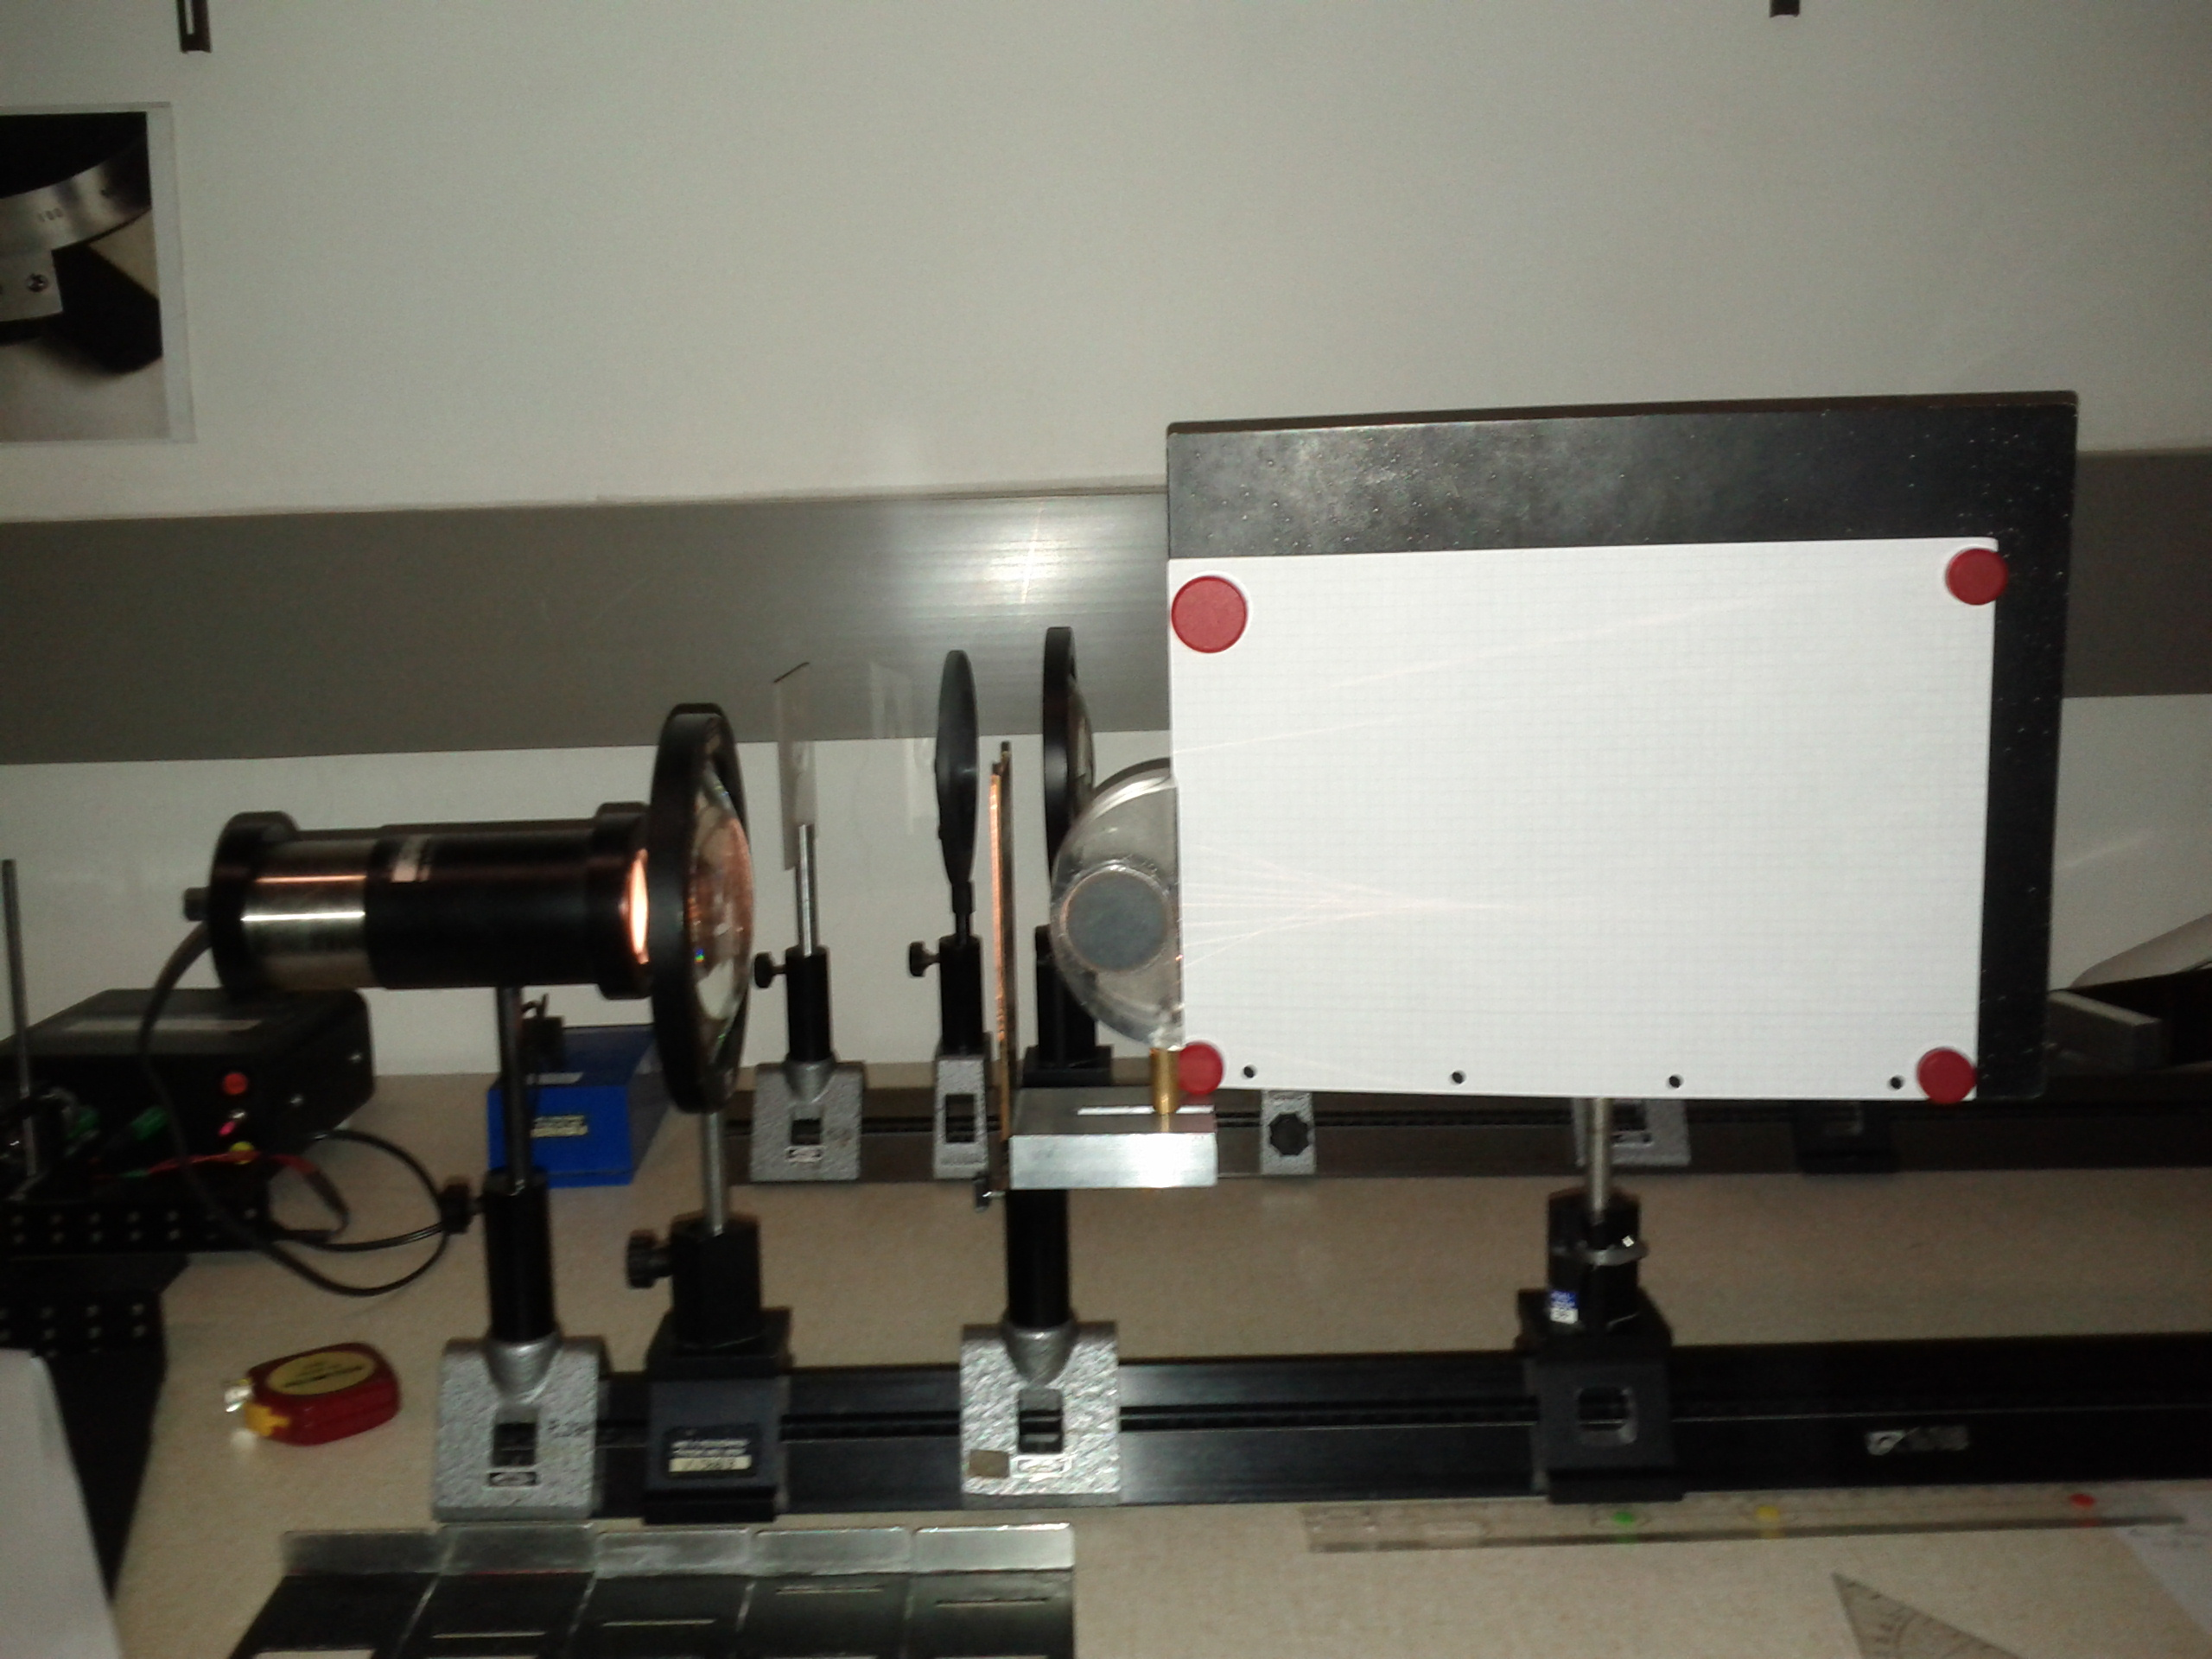
\includegraphics[scale=0.13]{./figure/linsenfehler.jpg}
%	\caption{Versuchaufbau Konvex-Plan Linse}
%	\label{fig:linsenfehler_aufbau}
%\end{figure}
%
%Glasprisma gegen Luft
%1.000292/sin(39grad28minutes)


%\begin{figure}[H]
%	\centering
%	\pgfplotstabletypeset[
%			columns={farbe, w,lambda},
%			col sep=&,
%			columns/farbe/.style={string type, column name=\makecell{$Farbe$\\} }, 
%			columns/w/.style={string type, column name=\makecell{$Winkel$\\$[Grad]$} }, 
%			columns/lambda/.style={column name=\makecell{$Wellenlänge$\\$[nm]$}, precision=0},
%			every head row/.style={before row=\hline,after row=\hline\hline},
%			every last row/.style={after row=\hline},
%			every first column/.style={column type/.add={|}{} },
%			every last column/.style={column type/.add={}{|} }
%			]{
%			farbe & w & lambda
%			rot & 47$^\circ$ 39' & 543
%			grün & 48$^\circ$ 58' & 508
%			zyan & 49$^\circ$ 29' & 479
%			blau & 49$^\circ$ 45' & 467
%			violett & 50$^\circ$ 18' & 441
%			
%			}
%	\caption{Farben, Winkel und Wellenlängen der Cadmium-Dampflampe}
%	\label{fig:werte_cadmiumdampflampe}
%\end{figure}



%%%%%%%%%%%%%%%%%%%%%%%%%%%%%%%%%%%%%%%%%%%%%%%%
\end{multicols}
\begin{figure}[H]
	\centering
	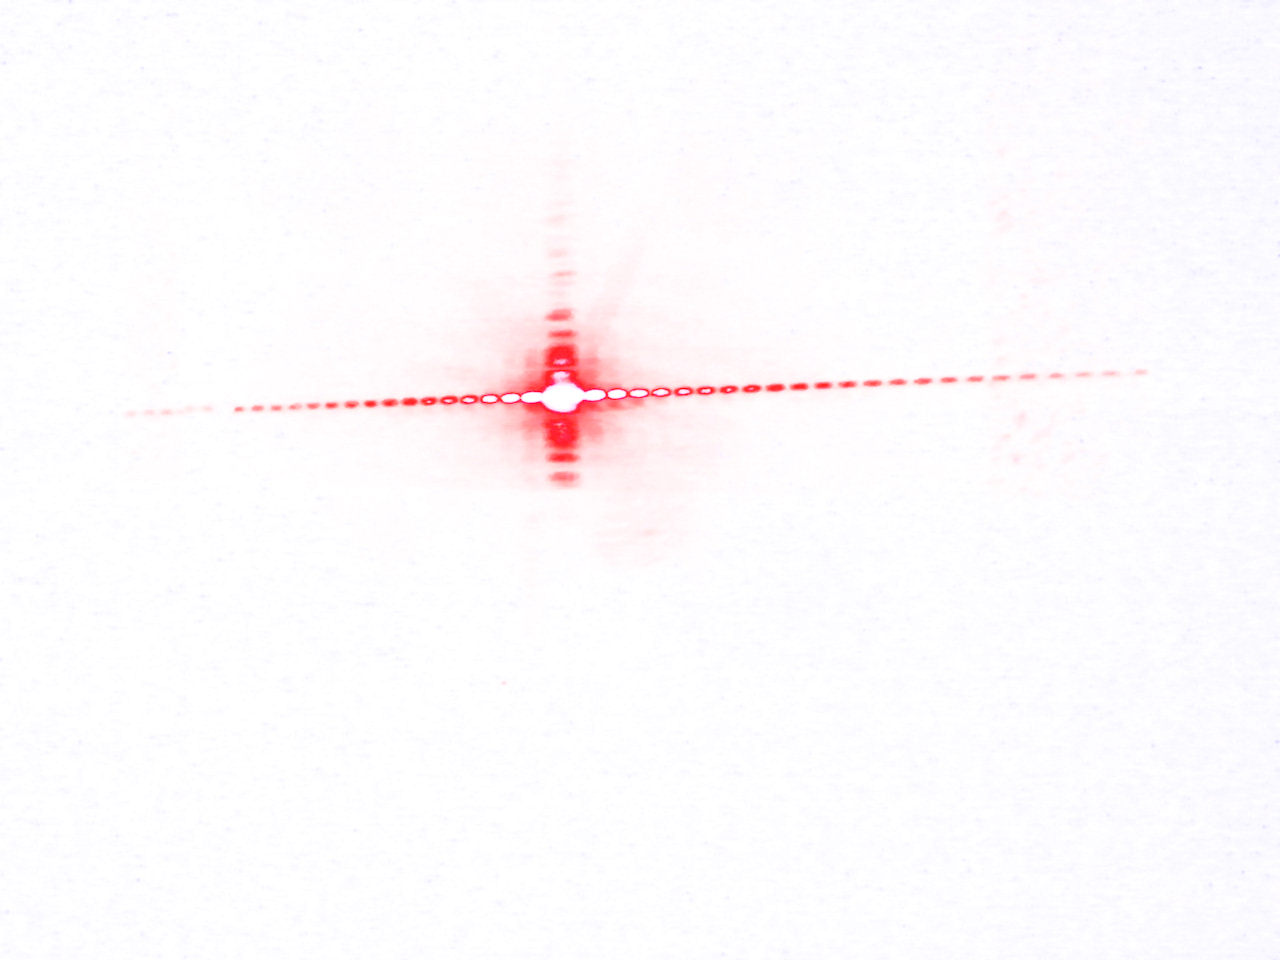
\includegraphics[scale=0.35]{./figure/beugung.png}
	\caption{Beugungsmuster Einzelspalt (echtes Foto; schwarz durch weiß ersetzt)}
	\label{fig:beugungsmuster}
\end{figure}

\begin{multicols}{2}

\section{Beugung am Spalt und Doppelspalt}
Im ersten Experiment soll ein Einzelspalt und ein Doppelspalt über die Beugung von monochromatischem Licht untersucht werden. Unsere Lichtquelle für monochromatisches Licht stellt ein roter Laser dar. Dadurch ergibt sich ein rotes Beugungsmuster auf dem Schirm (Abb. \ref{fig:beugungsmuster}). 
\\
Durch die Vermessung des Abstandes vom Einzelspalt zum Schirm (Abb. \ref{fig:messwerte_einzelspalt}) und dem Abstand zwischen den Minima kann direkt die Spaltbreite ermittelt werden [1](Glg. 13):
$$a = \frac{n*\lambda}{sin(\alpha_{min,n})} $$
$$\alpha_n = arctan(\frac{b_n}{R})$$
a...Spaltbreite\\
$b_n$...Abstand zwischen Minimum und 0-ter Ordnung\\
R...Abstand vom Spalt zum Schirm\\
$\lambda$...Wellenlänge des verwendeten Lichtes\\
\\
Beim Doppelspalt ergibt sich ein ähnliches Beugungsmuster nur das der Zentrale helle Punkt mehrere Minima und Maxima enthält. Durch eine Herleitung über die Beziehung zwischen Spaltbreite und Spaltabstand kann der Spaltabstand ermittelt werden:

$$ a = \frac{\lambda * n}{\alpha_n} $$
und
$$\frac{d}{a} = x$$
\noindent
x... Minima im Zentrum -1 halbiert\\
d... Spaltabstand (Mitte zu Mitte)\\
\\
Den Winkel erhalten wir wieder wie beim Einzelspalt.
Wesentlich in beiden Fällen ist das wir eine Fernfeldbeugung beobachten. Konkret muss der Abstand zum Beobachtungsschirm R folgender Gleichung genügen:
$$R \textgreater \frac{a^2}{\lambda}$$
\\
%d/a = x\\
%wobei: a = lambda*n/alpha_n (wellenlänge mal ordnung / gemessener winkel der jeweiligen ordnung)\\
%
%alpha_n = atan(messung/(2*R)) weil wir ja eine länge gemessen haben, in entfernung R... der faktor 1/2 kommt, weilma immer beide seiten gemessen und halbiert haben
%11 maxima -> x = 6

\subsection{Messwerte und Ergebnisse}

Wellenlänge des Laser der bei Einzel- und Doppelspalt verwendet wurde:
$$\lambda = 632.8nm$$

\end{multicols}
\begin{figure}[H]
	\centering
	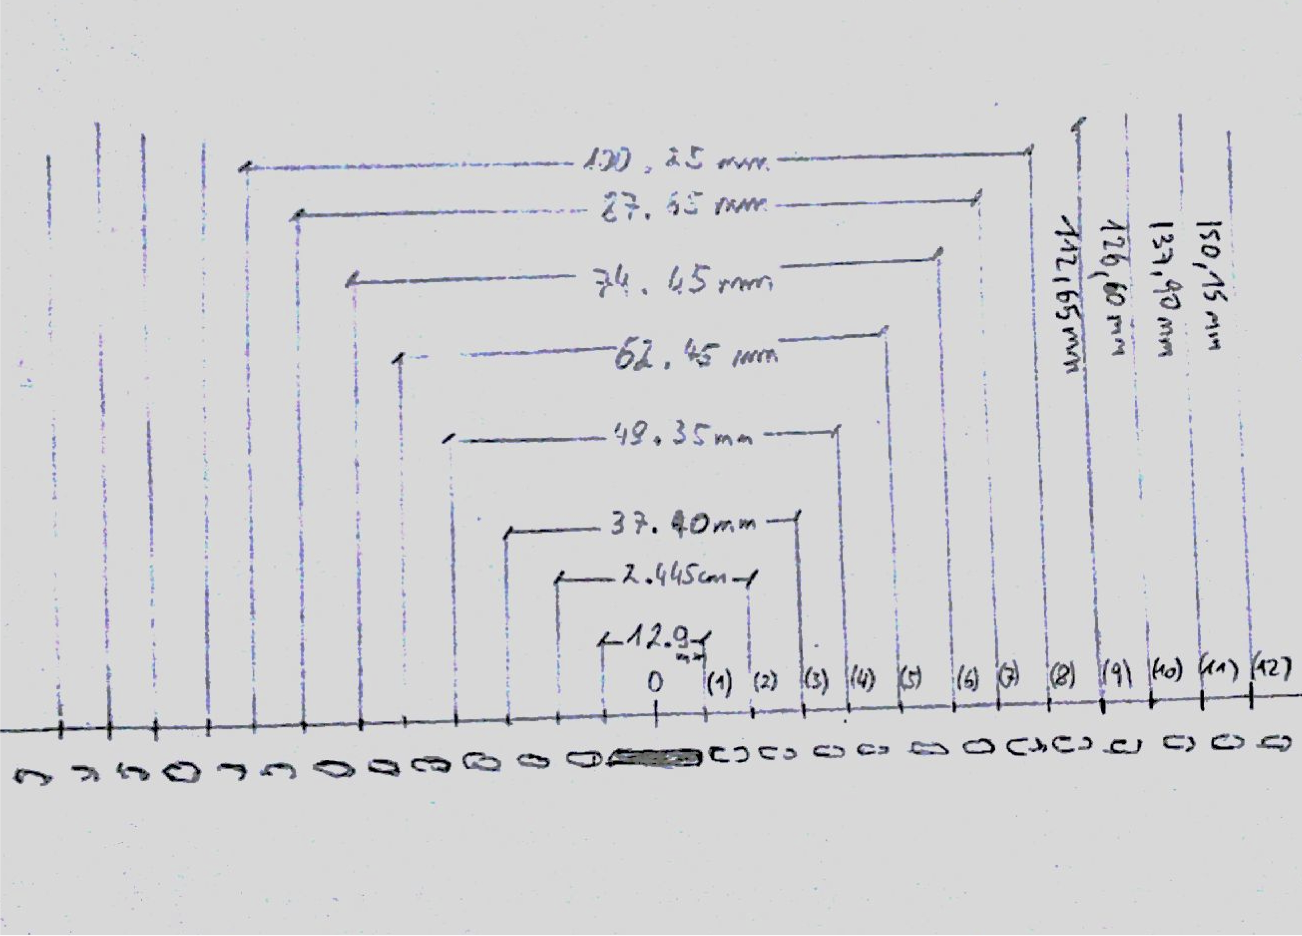
\includegraphics[scale=0.9]{./figure/einzelspalt_beugung.png}
	\caption{Beugungsmuster Einzelspalt mit Werten}
	\label{fig:messwerte_einzelspalt}
\end{figure}
\begin{figure}[H]
	\centering
	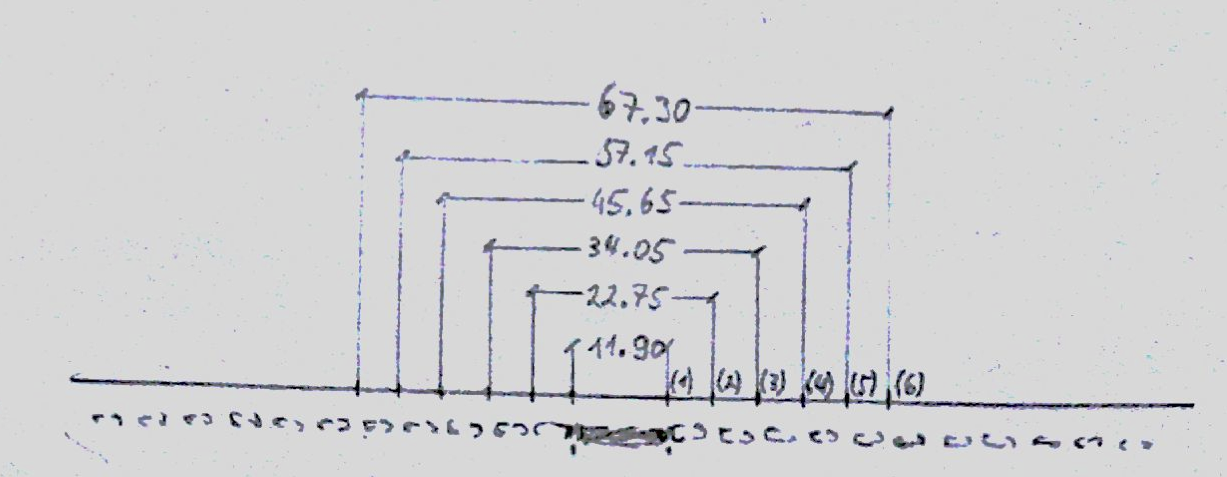
\includegraphics[scale=0.9]{./figure/doppelspalt_beugung.png}
	\caption{Beugungsmuster Doppelspalt mit Werten; ohne Minima und Maxima in der 0-ten Ordnung}
	\label{fig:messwerte_doppelspalt}
\end{figure}

\begin{multicols}{2}
\noindent
\textbf{Einzelspalt}\\
Mit den Messwerten aus \ref{tab:werte_doppelspalt} wurde mit den Formel aus der Einleitung in QTI-Plot eine Lineare Regression durchgeführt welche in Abbildung \ref{fig:einzelspalt_linreg} ersichtlich ist. 
\begin{figure}[H]
	\centering
	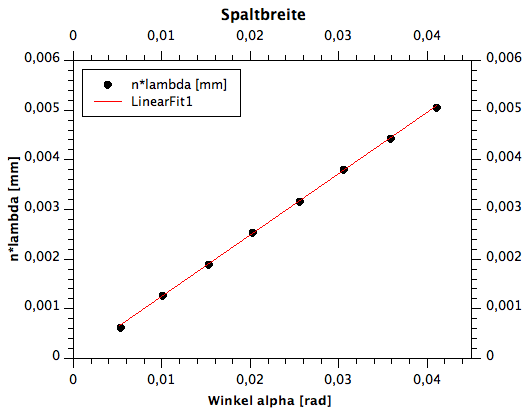
\includegraphics[scale=0.4]{./figure/linreg_einzelspalt.png}
	\caption{Lineare Regression Einzelspalt}
	\label{fig:einzelspalt_linreg}
\end{figure}
Daraus ergibt sich eine Spaltbreite von 
$$a = (0.1234 \pm 0.0065)mm$$
\begin{figure}[H]
	\centering
	\pgfplotstabletypeset[
			columns={abstand, n},
			col sep=&,
			columns/abstand/.style={precision=2, zerofill, column name=\makecell{$Abstand$\\$(\pm 0.05)[mm]$} }, 
			columns/n/.style={column name=\makecell{$n$\\$(Ordnung)$}, precision=0},
			every head row/.style={before row=\hline,after row=\hline\hline},
			every last row/.style={after row=\hline},
			every first column/.style={column type/.add={|}{} },
			every last column/.style={column type/.add={}{|} }
			]{
			abstand & n
			12.9 & 1
			24.45 & 2
			37.40 & 3
			49.35& 4
			62.45 & 5
			74.45 & 6
			87.45 & 7
			100.25 & 8
			
			}
	\caption{Messwerte Einzelspalt}
	\label{tab:werte_einzelspalt}
\end{figure}

\noindent
\textbf{Doppelspalt}\\
Wir konnten \textbf{11 Maxima} in der 0-ten Ordnung zählen was zu \textbf{x = 6} führt. 
Mit den Messwerten aus \ref{tab:werte_doppelspalt} wurde mit den Formel aus der Einleitung in QTI-Plot eine Lineare Regression durchgeführt welche in Abbildung \ref{fig:doppelspalt_linreg} ersichtlich ist. 
Zusätzlich musste der Abstand R gemessen werden um den Winkel zu berechnen:
$$R = (108.1 \pm 0.2)cm$$
Die Steigung ergibt folgende Spaltbreite:
$$a = (0.122 \pm 0.001)mm$$
\begin{figure}[H]
	\centering
	\pgfplotstabletypeset[
			columns={abstand, n},
			col sep=&,
			columns/abstand/.style={precision=2, zerofill, column name=\makecell{$Abstand$\\$(\pm 0.05)[mm]$} }, 
			columns/n/.style={column name=\makecell{$n$\\$(Ordnung)$}, precision=0},
			every head row/.style={before row=\hline,after row=\hline\hline},
			every last row/.style={after row=\hline},
			every first column/.style={column type/.add={|}{} },
			every last column/.style={column type/.add={}{|} }
			]{
			abstand & n
			11.9 & 1
			22.75 & 2
			34.05 & 3
			45.65& 4
			57.15 & 5
			67.30 & 6
			}
	\caption{Messwerte Doppelspalt}
	\label{tab:werte_doppelspalt}
\end{figure}
\begin{figure}[H]
	\centering
	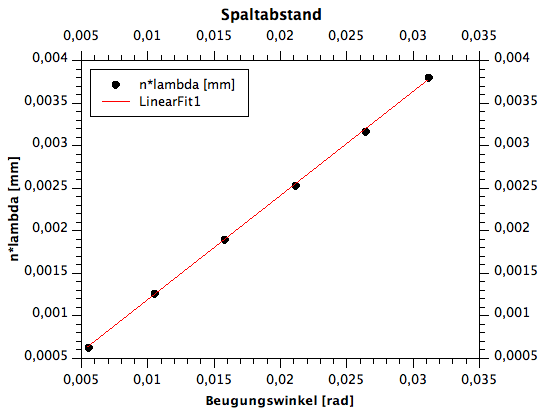
\includegraphics[scale=0.4]{./figure/linreg_doppelspalt.png}
	\caption{Lineare Regression Doppelspalt}
	\label{fig:doppelspalt_linreg}
\end{figure}
\noindent
Zu letzt ist noch der Spaltabstand mit der Formel 
$$\frac{d}{a} = x$$
\noindent
zu berechnen.
$$d = x*a = 6 * 0.122 = (0.732 \pm 0.001)mm$$

\subsection{Diskussion}
Die Ausrichtung des Lasers auf den Spalt gestaltete sich etwas wackelig, da der Laser per Hand gedreht wurde. Nach wenigen Versuchen war jedoch ein brauchbares Muster am Schirm zu erkennen. Die Messfehler durch Schublehre und Maßband waren erstaunlich gering, was mit der zusätzlichen Regression zu einem guten Ergebnis geführt hat.\\
Beim Doppelspalt war eine genaue Einstellung des Lasers nur bei absoluter Dunkelheit und gleichzeitiger Beobachtung der 0-ten Ordnung erfolgreich, da bei einer kleinen Abweichung bereits die Minima und Maxima verschwimmen. Trotz guter Justierung konnten bei den ersten Zählungen nur 9 statt 11 Maxima gesehen werden.  

%%%%%%%%%%%%%%%%%%%%%%%%%%%%%%%%%%%%%%%%%%%%%%%%
\section{Wellenlängenmessung am Gitter}



\subsection{Messwerte und Ergebnisse}




\subsection{Diskussion}


%%%%%%%%%%%%%%%%%%%%%%%%%%%%%%%%%%%%%%%%%%%%%%%%
\section{Newtonsche Ringe}


\subsection{Messwerte und Ergebnisse}



\subsection{Diskussion}

\section{Quellen}
$[1]$ Leitfaden, \url{http://www.univie.ac.at/anfpra/neu1/pw/pw8/PW8.pdf}\\
%$[2]$

\end{multicols}
\end{document}